
\section{Besondere Anlässe}
\label{section:besondere_anlaesse}
\begin{frame}%STARTCONTENT

\begin{columns}
    \begin{column}{0.48\textwidth}
    
\begin{figure}
    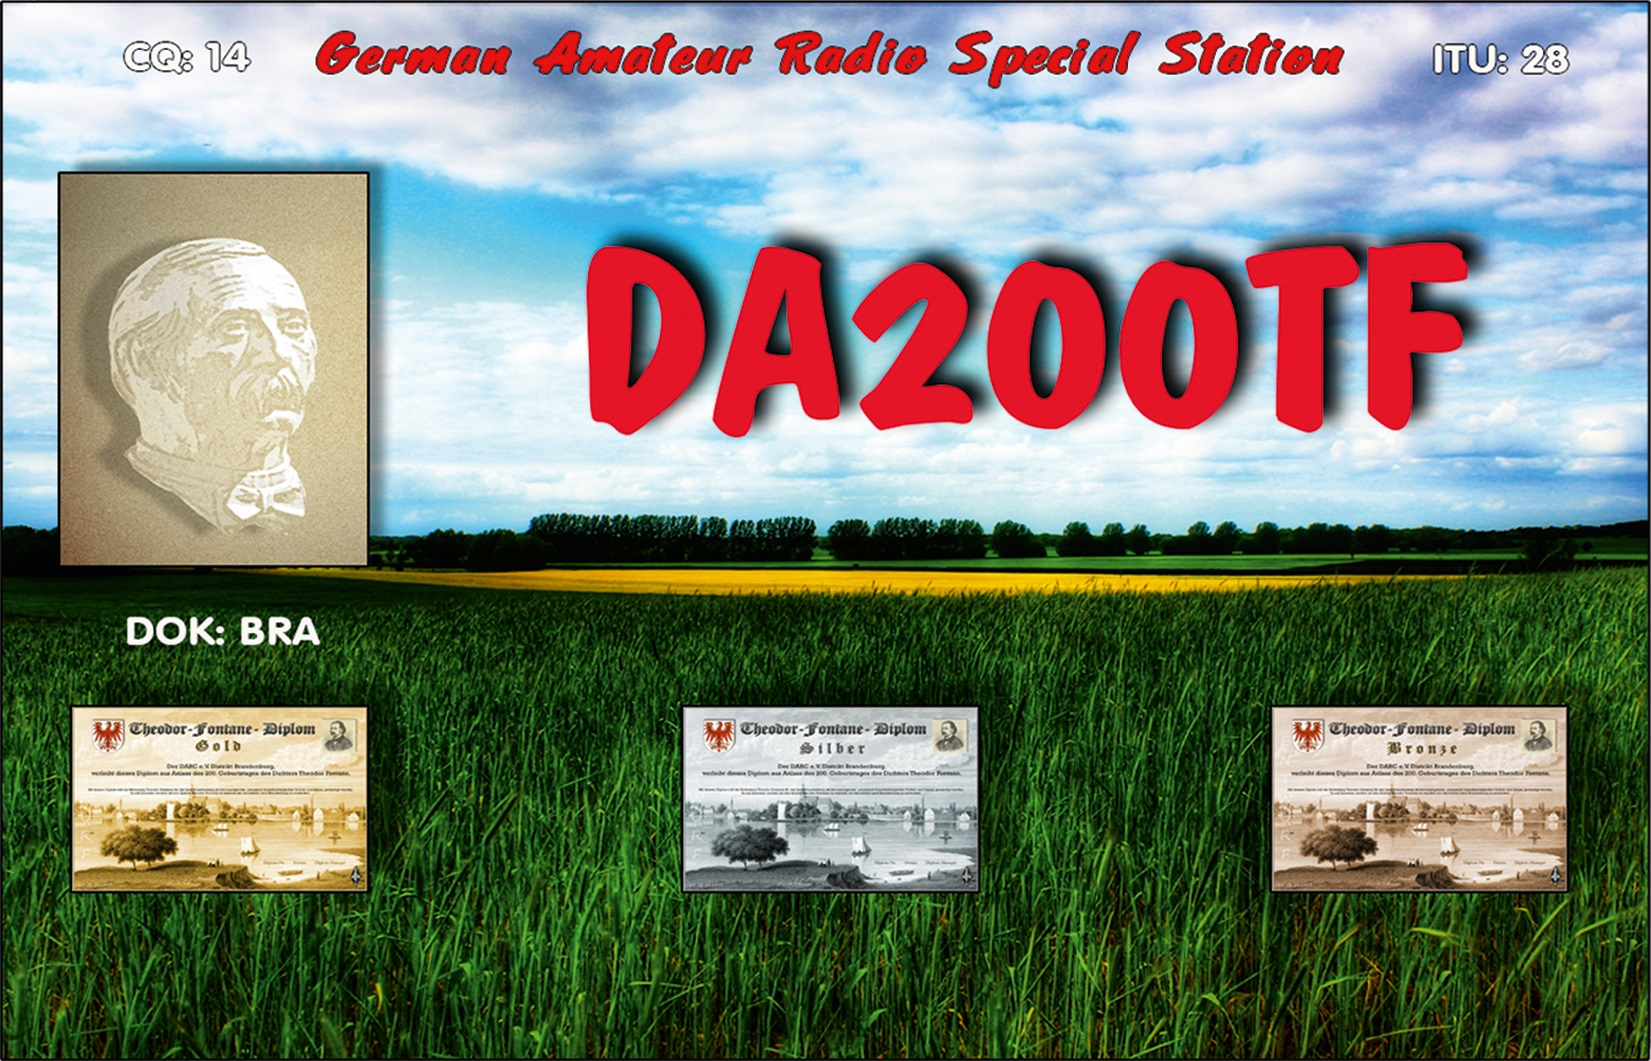
\includegraphics[width=0.85\textwidth]{foto/59}
    \caption{\scriptsize QSL-Karte der Klubstation mit dem Sonderrufzeichen DA200TF anlässlich des 200. Geburtstag von Theodor Fontane}
    \label{n_besondere_anlaesse_qsl_karte_DA200TF}
\end{figure}

    \end{column}
   \begin{column}{0.48\textwidth}
       \begin{itemize}
  \item Klubstationsrufzeichen mit 4-7stelligem Suffix
  \item z.B. für historische Ereignisse, Stadtfeste oder Sportereignisse
  \item Die ganze Amateurfunkwelt kann an dem Ereignis teilhaben
  \end{itemize}

   \end{column}
\end{columns}

\end{frame}

\begin{frame}
\frametitle{Vorgaben}
\begin{itemize}
  \item Maximale Zuweisung für 1 Jahr durch die BNetzA
  \item Keine Verlängerung möglich
  \item Suffix kann aus Ziffern und Buchstaben bestehen
  \item Das letzte Zeichen muss immer ein Buchstabe sein
  \end{itemize}
\end{frame}

\begin{frame}
\frametitle{International}
\begin{itemize}
  \item Auch im Ausland kann es Sonderstationen geben
  \item Die Rufzeichen können andere Vorgaben haben
  \end{itemize}
\end{frame}

\begin{frame}\begin{table}
\begin{DARCtabular}{llX}
     Rufzeichen  & Zuteilung  & Ereignis   \\
     DL1250BRET  & 2017  & 1250 Jahre Stadt Bretten   \\
     DL500BIER  & 2016  & 500 Jahre Deutsches Reinheitsgebot   \\
     DF13DEJU  & 2019  & Erstflug der Junkers F 13   \\
     DL73AFUG  & 2022  & 73. Geburtstags des Amateurfunkgesetzes   \\
     DB50AFZ  & 2022  & 50 Jahre Amateurfunkzentrum   \\
     DP44N44T  & 2022  & 44 Jahre Ortsverband N44   \\
     DC0YOTA  & 2021  & Youngsters On The Air   \\
     DL22MAUS  & 2022  & Türen auf mit der Maus!   \\
     DL0ELEFANT  & 2022  & Türen auf mit der Maus!   \\
\end{DARCtabular}
\caption{Beispiele für Sonderstationen}
\label{n_besondere_anlaesse}
\end{table}

\end{frame}

\begin{frame}
\only<1>{
\begin{QQuestion}{VD204}{Warum ist \glqq DL250BTHVN\grqq{} ein zulässiges deutsches Amateurfunkrufzeichen?}{Weil für besonders verdiente Funkamateure auch personengebundene Rufzeichen ausgegeben werden, für die der Rufzeichenplan keine Anwendung findet.}
{Weil der Rufzeichenplan zu besonderen allgemeinen Anlässen auch Rufzeichen mit bis zu 7 Zeichen langem Suffix vorsieht, der Ziffern enthalten kann und mit einem Buchstaben endet.}
{Weil an bestimmte öffentliche Stellen, wie z.~B. Kunst- und Kultureinrichtungen, besondere Rufzeichen mit mindestens 3 Ziffern ausgegeben werden.}
{Weil dies in einer Sonderverfügung der Bundesnetzagentur aufgrund besonderen historischen Anlass mit internationaler Wirkung festgelegt wurde.}
\end{QQuestion}

}
\only<2>{
\begin{QQuestion}{VD204}{Warum ist \glqq DL250BTHVN\grqq{} ein zulässiges deutsches Amateurfunkrufzeichen?}{Weil für besonders verdiente Funkamateure auch personengebundene Rufzeichen ausgegeben werden, für die der Rufzeichenplan keine Anwendung findet.}
{\textbf{\textcolor{DARCgreen}{Weil der Rufzeichenplan zu besonderen allgemeinen Anlässen auch Rufzeichen mit bis zu 7 Zeichen langem Suffix vorsieht, der Ziffern enthalten kann und mit einem Buchstaben endet.}}}
{Weil an bestimmte öffentliche Stellen, wie z.~B. Kunst- und Kultureinrichtungen, besondere Rufzeichen mit mindestens 3 Ziffern ausgegeben werden.}
{Weil dies in einer Sonderverfügung der Bundesnetzagentur aufgrund besonderen historischen Anlass mit internationaler Wirkung festgelegt wurde.}
\end{QQuestion}

}
\end{frame}%ENDCONTENT
